\begin{figure}[htbp]
\centering
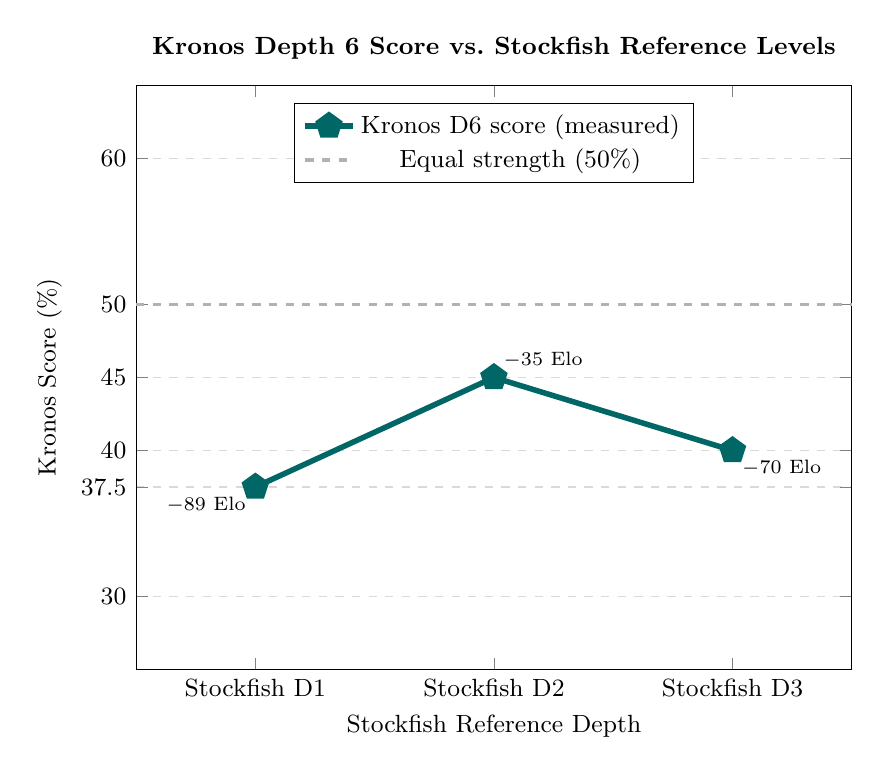
\begin{tikzpicture}
\begin{axis}[
    title style={font=\bfseries\small},
    title={Kronos Depth 6 Score vs.\ Stockfish Reference Levels},
    xlabel={Stockfish Reference Depth},
    ylabel={Kronos Score (\%)},
    xmin=0.5, xmax=3.5,
    ymin=25, ymax=65,
    xtick={1,2,3},
    xticklabels={Stockfish D1, Stockfish D2, Stockfish D3},
    ytick={30,37.5,40,45,50,60},
    ymajorgrids=true,
    grid style={dashed, gray!30},
    width=0.88\textwidth,
    height=9cm,
    tick label style={font=\small},
    label style={font=\small},
    legend style={font=\small, at={(0.5,0.97)}, anchor=north}
]

% Measured calibration scores
\addplot[
    color=teal!80!black,
    mark=pentagon*,
    mark size=4pt,
    line width=2pt
]
coordinates {
    (1, 37.5)
    (2, 45.0)
    (3, 40.0)
};
\addlegendentry{Kronos D6 score (measured)}

% 50% reference line as explicit coordinates
\addplot[
    dashed,
    color=gray!60,
    line width=1.2pt
]
coordinates {
    (0.5, 50)
    (3.5, 50)
};
\addlegendentry{Equal strength (50\%)}

% Annotate each point
\node[font=\scriptsize, anchor=north east] at (axis cs:1,37.5) {$-$89 Elo};
\node[font=\scriptsize, anchor=south west] at (axis cs:2,45.0) {$-$35 Elo};
\node[font=\scriptsize, anchor=north west] at (axis cs:3,40.0) {$-$70 Elo};

\end{axis}
\end{tikzpicture}
\caption[Stockfish Calibration Results]{Kronos Depth 6 match score against three depth-limited Stockfish 18 configurations. Scores below 50\% indicate that Stockfish outperforms Kronos at all tested depths. Speculative projections are moved to Appendix~\ref{app:sf_projections}.}


\label{fig:stockfish_calibration}
\end{figure}
% Source Material: stockfish_calibration.tex measured rows only
